En este cap�tulo se definen los par�metros a controlar tomando el sistema de segundo orden expuesto en el cap�tulo \ref{CAP:accio} y as� estimar la respuesta con el polo deseado.
%se debe buscar los par�metros a controlar para obtener la respuesta del polo deseado.

\section{Respuesta del sistema ante un escal�n unitario}

Al estudiar el sistema de segundo orden en el cap�tulo \ref{CAP:accio}, se observa que la respuesta al escal�n unitario da como resultado la figura \ref{fig:escalon}:



\begin{figure}[H]
	\centering
	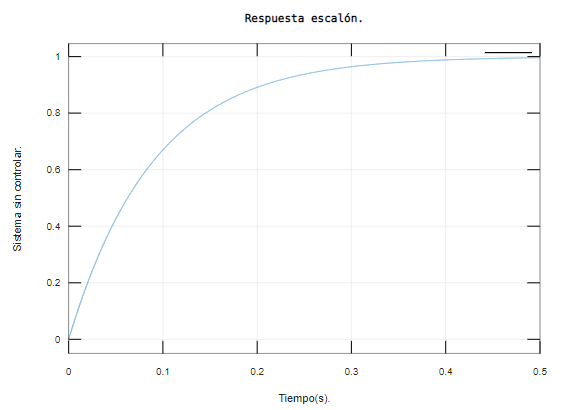
\includegraphics[width=0.7\linewidth]{img/escalon}
	\caption{Respuesta escal�n}
	\label{fig:escalon}
\end{figure}
 
Se utiliza una funci�n escal�n ya que est� representa un cambio instantaneo la entrada de referencia, este hace que revele qu� tan rapido responde un sistema a entradas con cambios abruptos.

Se debe tomar en cuenta algunos criterios de dise�os utilizados para la caracterizaci�n de los sistemas de control lineales en el dominio del tiempo:


\begin{itemize}
	\item \textbf{Sobrepico m�ximo:} Si se define y(t) la respuesta del escal�n unitario, $y_{ss}$ el valor en estado estable de y(t) y $y_{max}$ el valor m�ximo de la misma, entonces el sobrepico m�ximo se define como:
	
		\begin{center}
				$Sobrepico= y_{max}-y_{ss}$
		\end{center}
	
	El sobrepico se representa como un porcentaje del valor final, expuesto en la ecuaci�n \ref{ec:sobrepico}:
	
		\begin{center}
		\begin{equation}\label{ec:sobrepico}
			\%Sobrepico=\dfrac{Sobrepico}{y_{ss}}*100
		\end{equation}
	\end{center}
	
	El sobrepico se utiliza para medir la estabilidad relativa del sistema de control por este motivo un  sobrepico alto es indeseable.
	
	\item \textbf{Tiempo de retardo $t_{d}$:} Es el tiempo que se necesita para que la respuesta escal�n alcance el 50$\%$  del valor final de la gr�fica.
	
   \item \textbf{Tiempo de alza $t_{r}$:} Es el tiempoo que toma la respuesta escal�n se eleve del 10 al 90$\%$ del valor final.
   
   \item \textbf{Tiempo de establecimiento $t_{s}$:} Es el tiempo que se requiere para que la respuesta escal�n  disminuya y permanezca dentro de un rango del valor final. Un valor frecuente que se utiliza es 5$\%$ y se calcula \ref{ec:ts}.
   
   \begin{center}
   	\begin{equation}\label{ec:ts}
   		 T_{s}=3\tau=\frac{3}{\zeta\omega_{n}}
   	\end{equation}
   \end{center}
   
\end{itemize}


Para ejemplificar mejor todos los criterios antes mencionados se muestra la imagen \ref{fig:escalon1}

\begin{figure}[H]
	\centering
	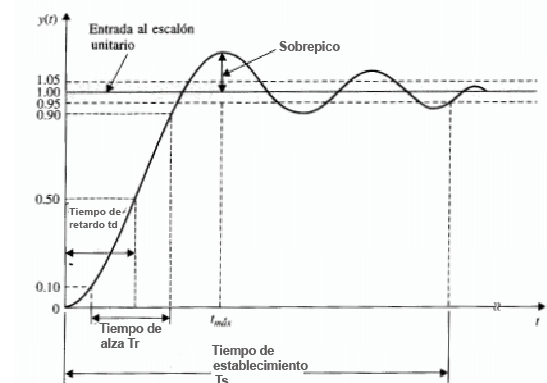
\includegraphics[width=0.7\linewidth]{img/imagenescalonej}
	\caption{Respuesta t�pica al escal�n unitario de un sistema de control}
	\cite{kuo}
	\label{fig:escalon1}
\end{figure}

Como ya se ha mencionado en los cap�tulo \ref{CAP:tecni} los sistemas de control de segundo orden con realimentaci�n unitaria a lazo cerrado se representa en la ecuaci�n \ref{ec:segundoorden}


\begin{center}
	$	F(s)=\frac{\omega_{n}^{2}}{s^{2}+2\zeta \omega_{n}s+\omega_{n}^{2}}$
\end{center}

El factor de amortiguamiento $\zeta$ y la frecuencia natural $\omega_{n}$ constituyen las ra�ces de la ecuaci�n caracter�stica. Cuando $\zeta \geq 1$ la respuesta escal�n no muestra sobrepicos,  si $0< \zeta < 1$ entonces el sistema es subamortiguado y si $\zeta=o $ el amortiguamiento es cero, el sistema se vuelve cr�ticamente estable. Las dos ra�ces se pueden expresar:

\begin{center}
	\begin{equation}\label{raices}
		S_{1},S_{2}=-\zeta\omega_{n}\pm j\omega_{n}\sqrt{1-\zeta^{2}}
	\end{equation}
\end{center}


